\clearpage
\begin{savequote}[8cm]
\textlatin{Neque porro quisquam est qui dolorem ipsum quia dolor sit amet, consectetur, adipisci velit...}

There is no one who loves pain itself, who seeks after it and wants to have it, simply because it is pain...
  \qauthor{--- Cicero's \textit{de Finibus Bonorum et Malorum}}
\end{savequote}

\chapter{\label{ch:6-interpretation}Extraction of CKM angle \Pgamma} 

\minitoc

The equations \ref{exp_Acp}, \ref{exp_Rcp} and \ref{exp_Rpm} are used to relate physics observables to physics parameters. 

\section{Coherence factor}
\label{sec:interpretation:coherence}

The $K^*$ has a large natural width (about 50 MeV), therefore non-resonant processes may be non-neglibigle, which would affect the measurement of \Pgamma. Due to the large natural width, the amplitudes and phases of the different decays may be different at each point in phasespace:

\begin{align*}
A(B^- \to D^0 K^{*-}) &= A_c(p) e^{i\delta_c(p)} \\
A(B^- \to \bar{D^0} K^{*-}) &= A_u(p) e^{i\delta_u(p) e^{-i\gamma}} \\
A(D^0 \to K^-\pi^+) &= A_{K\pi} e^{i\delta_{K\pi}} \\
A(D^0 \to K^+\pi^-) &= A_{{\pi}K} e^{i\delta_{{\pi}K}} 
\end{align*}

\begin{align*}
r_s &= \frac{\Gamma(B^- \to \bar{D^0}K^{*-})}{\Gamma(B^- \to D^0K^{*-})} = \frac{\int \left|A_u(p)\right|^2 \mathrm{d}p}{\int \left|A_c(p)\right|^2 \mathrm{d}p}
\end{align*}

\begin{align}
\kappa e^{i\delta_s} &= \frac{\int \mathrm{d}p A_c(p)A_u(p)e^{i\delta(p)}}{\sqrt{\int \mathrm{d}p \left|A_u(p)\right|^2 \int \mathrm{d}p \left|A_c(p)\right|^2}}
\label{kappadefinition}
\end{align}

where p represents a point in phasespace, and $0 \leq \kappa \leq 1$ and $0 \leq \delta_s \leq 2\pi$. The amplitudes include both resonant $B^- \to DK^{*-}$ and non-resonant contributions, which is what the $\kappa$ factor accounts for.

Using this formalism it can be shown that the $\kappa$ factor can be included in the expressions of the CP observables as shown in Equations \ref{exp_Acp}, \ref{exp_Rcp} and \ref{exp_Rpm}. The value for $\kappa$ can be estimated and then used alongside the CP observables to extract \Pgamma, $r_B$ and $\delta_B$.

\subsection{Decay model}
\label{sec:interpretation:model}

The components of the model used for this study are:

\begin{itemize}
\item $\decay{\Bp}{\Dz K^*(892)^+}$ and $\decay{\Bp}{\Dzb K^*(892)^+}$
%\item $\decay{\Bp}{\Dz K^*(1410)^+}$ and $\decay{\Bp}{\Dzb K^*(1410)^+}$
\item $\decay{\Bp}{\Dz K^*_0(1430)^+}$ and $\decay{\Bp}{\Dzb K^*_0(1430)^+}$
\end{itemize}

A non resonant LASS component is used in the model, which is part of the $K^*_0(1430)^+$. Other resonances e.g. $K^*(1680)^+$ and $D_2^*(2460)^-$, are considered to be negligible in the region being considered and so are not included in the decay model. The parameters of the resonances are listed in Table \ref{resonances}.

\begin{table}[h]
\centering
\begin{tabular}{llll}
\hline
Resonance & Mass, M \mev & Width, $\Gamma$ \mev & Spin \\
\hline
$K^*(892)^+$ & $891.66 \pm 0.26$ & $50.8 \pm 0.9$ & 1 \\
%$K^*(1410)^+$ & $1414 \pm 15$ & $232 \pm 21$ & 1 \\
$K^*_0(1430)^+$ & $1425 \pm 50$ & $270 \pm 80$ & 0 \\
\hline
\end{tabular}
\caption{Parameters of the resonances in the decay model}
\label{resonances}
\end{table}

The ampltiude model was generated using the Laura++ package~\cite{Laura}. The amplitudes $A_{\uquark\bquark}$ and $A_{\cquark\bquark}$ are taken as,

\begin{align*}
A_{\uquark\bquark} =\ & a_{\uquark\bquark}^{K^*(892)^+}e^{-i\delta_{\uquark\bquark}^{K^*(892)^+}}RelBW(p;M_{K^*(892)^+},\Gamma_{K^*(892)^+},1)\ + \\
& a_{\uquark\bquark}^{K^*_0(1430)^+}e^{-i\delta_{\uquark\bquark}^{K^*_0(1430)^+}}LASS\_BW(p;M_{K^*_0(1430)^+},\Gamma_{K^*_0(1430)^+},0)\ + \\
& a_{\uquark\bquark}^{NR}e^{-i\delta_{\uquark\bquark}^{NR}}LASS\_NR
\end{align*}

and

\begin{align*}
A_{\cquark\bquark} =\ & a_{\cquark\bquark}^{K^*(892)^+}e^{-i\delta_{\cquark\bquark}^{K^*(892)^+}}RelBW(p;M_{K^*(892)^+},\Gamma_{K^*(892)^+},1)\ + \\
& a_{\cquark\bquark}^{K^*_0(1430)^+}e^{-i\delta_{\cquark\bquark}^{K^*_0(1430)^+}}LASS\_BW(p;M_{K^*_0(1430)^+},\Gamma_{K^*_0(1430)^+},0)\ + \\
& a_{\cquark\bquark}^{NR}e^{-i\delta_{\cquark\bquark}^{NR}}LASS\_NR
\end{align*}

where, $RelBW$, $LASS\_BW$ and $LASS\_NR$ refer to the relativistic Breit-Wigner, LASS Breit-Wigner and LASS non-resonance shapes as implemented in Laura++~\cite{Laura}. 

The relative square of the magnitude of the various components is equal to the relative branching fractions in the limit of no interference. Therefore, it is assumed that the relative ampltitudes are equal to the relative branching fractions. The only available branching fraction measurement is,

\begin{equation*}
\BF(\decay{\Bp}{\Dzb K^*(892)^+}) \times \BF(\decay{K^*(892)^+}{\KS\pip}) = 1.8 \times 10^{-4}
\end{equation*}

For the \Kstar modes, it is assumed that they are produced with the same branching fraction as the $K^*(892)$ mode, and the branching fraction to $K\pi$ is taken into account.

\begin{itemize}
\item $\BR(\decay{K^*(892)^+}{\KS\pip}) = \frac{1}{3}$
%\item $\BR(\decay{K^*(1410)^+}{\KS\pip}) = 0.022$
\item $\BR(\decay{K^*_0(1430)^+}{\KS\pip}) = 0.31$
\end{itemize}

The non-resonant branching fraction \BR(\decay{\Bp}{\Dzb\KS\pip}) is not known, so the branching fraction ratio,

\begin{equation*}
\frac{\BR(\decay{\Bz}{\Dm\Kz\pip})}{\BR(\decay{\Bz}{\Dm\Kzb\Kp})} = 1.6 \pm 0.3
\end{equation*}

is assumed to equal to,

\begin{equation*}
\frac{\BR(\decay{\Bp}{\Dzb\Kz\pip})}{\BR(\decay{\Bp}{\Dzb\Kzb\Kp})}
\end{equation*}

where $\BR(\decay{\Bp}{\Dzb\Kzb\Kp}) = (5.5 \pm 1.6) \times 10^{-4}$~\cite{PDG2014}.

When generating an amplitude model we are only interested the relative amplitudes and phases of the various components, therefore the $K^*(892)$ is fixed to have an amplitude of 1 and phase of 0. The relative amplitude $r_B$ is assumed to be 0.1. The values of the squares of the amplitudes $a_{\uquark\bquark}$ and $a_{\cquark\bquark}$ of the Breit-Wigner functions are taken in the ranges:

\begin{itemize}
\item \textbar $a_{\cquark\bquark}^{K^*(892)^+}$\textbar$^2 = 1$
%\item \textbar $a_{\cquark\bquark}^{K^*(1410)^+}$\textbar$^2 \in [0.7 \times 0.066,1.3 \times 0.066]$
\item \textbar $a_{\cquark\bquark}^{K^*_0(1430)^+}$\textbar$^2 \in [0.7 \times 0.93,1.3 \times 0.93]$
\item \textbar $a_{\cquark\bquark}^{NR}$\textbar$^2 \in [0.0,2.4]$
\end{itemize}

and,

\begin{itemize}
\item $a_{\uquark\bquark}^{K^*(892)^+} = r_B a_{\cquark\bquark}^{K^*(892)^+}$
%\item $a_{\uquark\bquark}^{K^*(1410)^+} = r_B a_{\cquark\bquark}^{K^*(1410)^+}$
\item $a_{\uquark\bquark}^{K^*_0(1430)^+} = r_B a_{\cquark\bquark}^{K^*_0(1430)^+}$
\item $a_{\uquark\bquark}^{NR} = r_B a_{\cquark\bquark}^{NR}$
\end{itemize}

Figure \ref{dalitzplot} shows an example Dalitz plot used in the toys. The \Kstar selection in this analysis, \Kstar mass window and \KS helicity angle, are represented by dashed lines in this plot.

\begin{figure}[h]
\centering
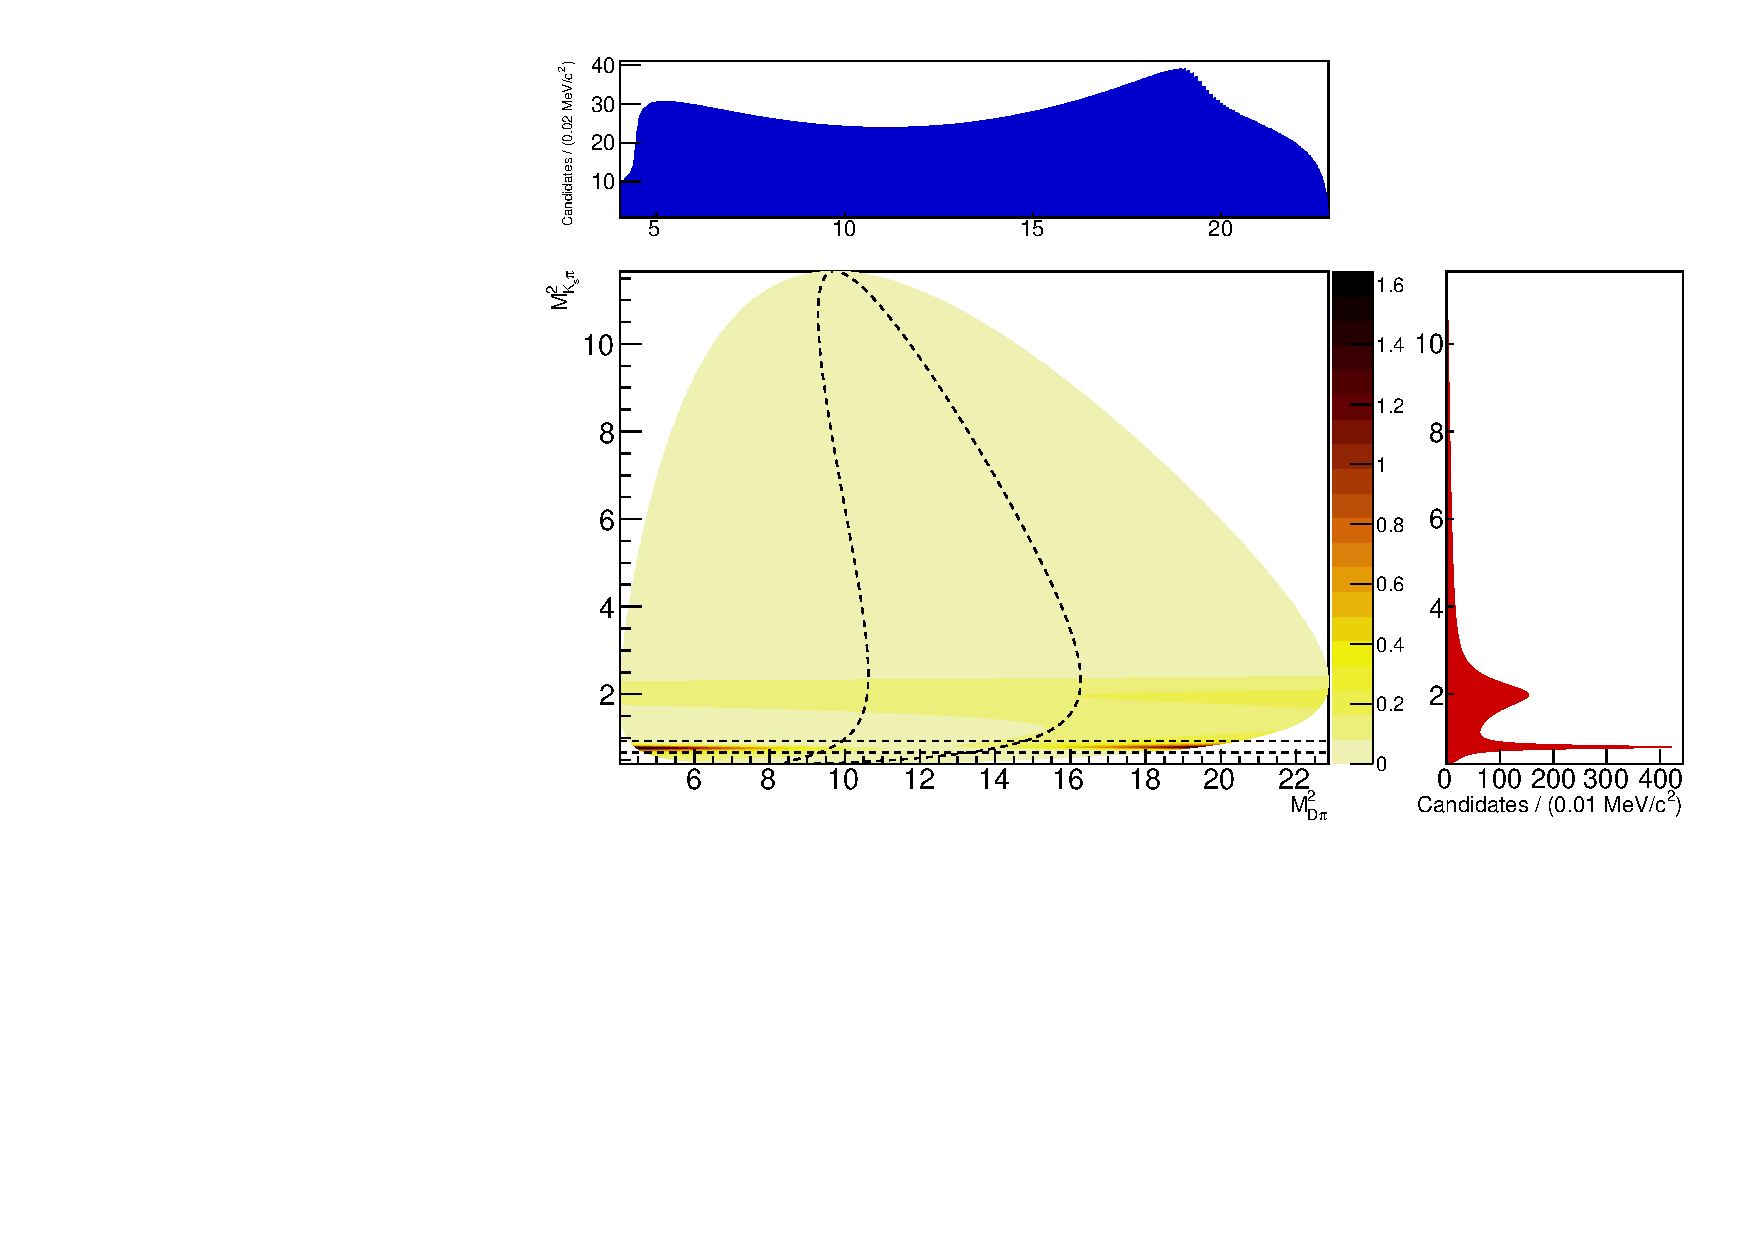
\includegraphics[width=0.8\linewidth]{figures/results/dalitz.pdf}
\caption{Example dalitz plot used in the toys. The projections in the two dalitz plot coordinates are shown. The dashed lines on the Dalitz plot represent the \Kstar mass and \KS helicity angle selection used in this analysis.}
\label{dalitzplot}
\end{figure}

\subsection{Estimation of $\kappa$}

A large number of toy Dalitz plots (1000) are generated varying the ampltiudes and phases of the different resonances within limits as descibed by the decay model. The limits for the amplitudes are given in Seciton \ref{sec:interpretation:model} and all phases are generated randomly according to a falt distribution between $-\pi$ and $\pi$. Masses and widths of the resonances are kept constant at their central values. 

For each Dalitz plot $\kappa$ is computed as the magnitude of the expression in Equation \ref{kappadefinition}. The mean and standard deviation of the resulting distribution is taken as an estimate of the central value and uncertainty of $\kappa$. The resulting distribution is shown in Figure \ref{kappadistribution} and gives an estimate for $\kappa$ of $0.95 \pm 0.04$. The uncertainty of this distribution is enhanced to account for the skewness of the distribution, therefore a final value of $0.95 \pm 0.06$ is used in order to extract the physics parameters of interest.

\begin{figure}[h]
\centering
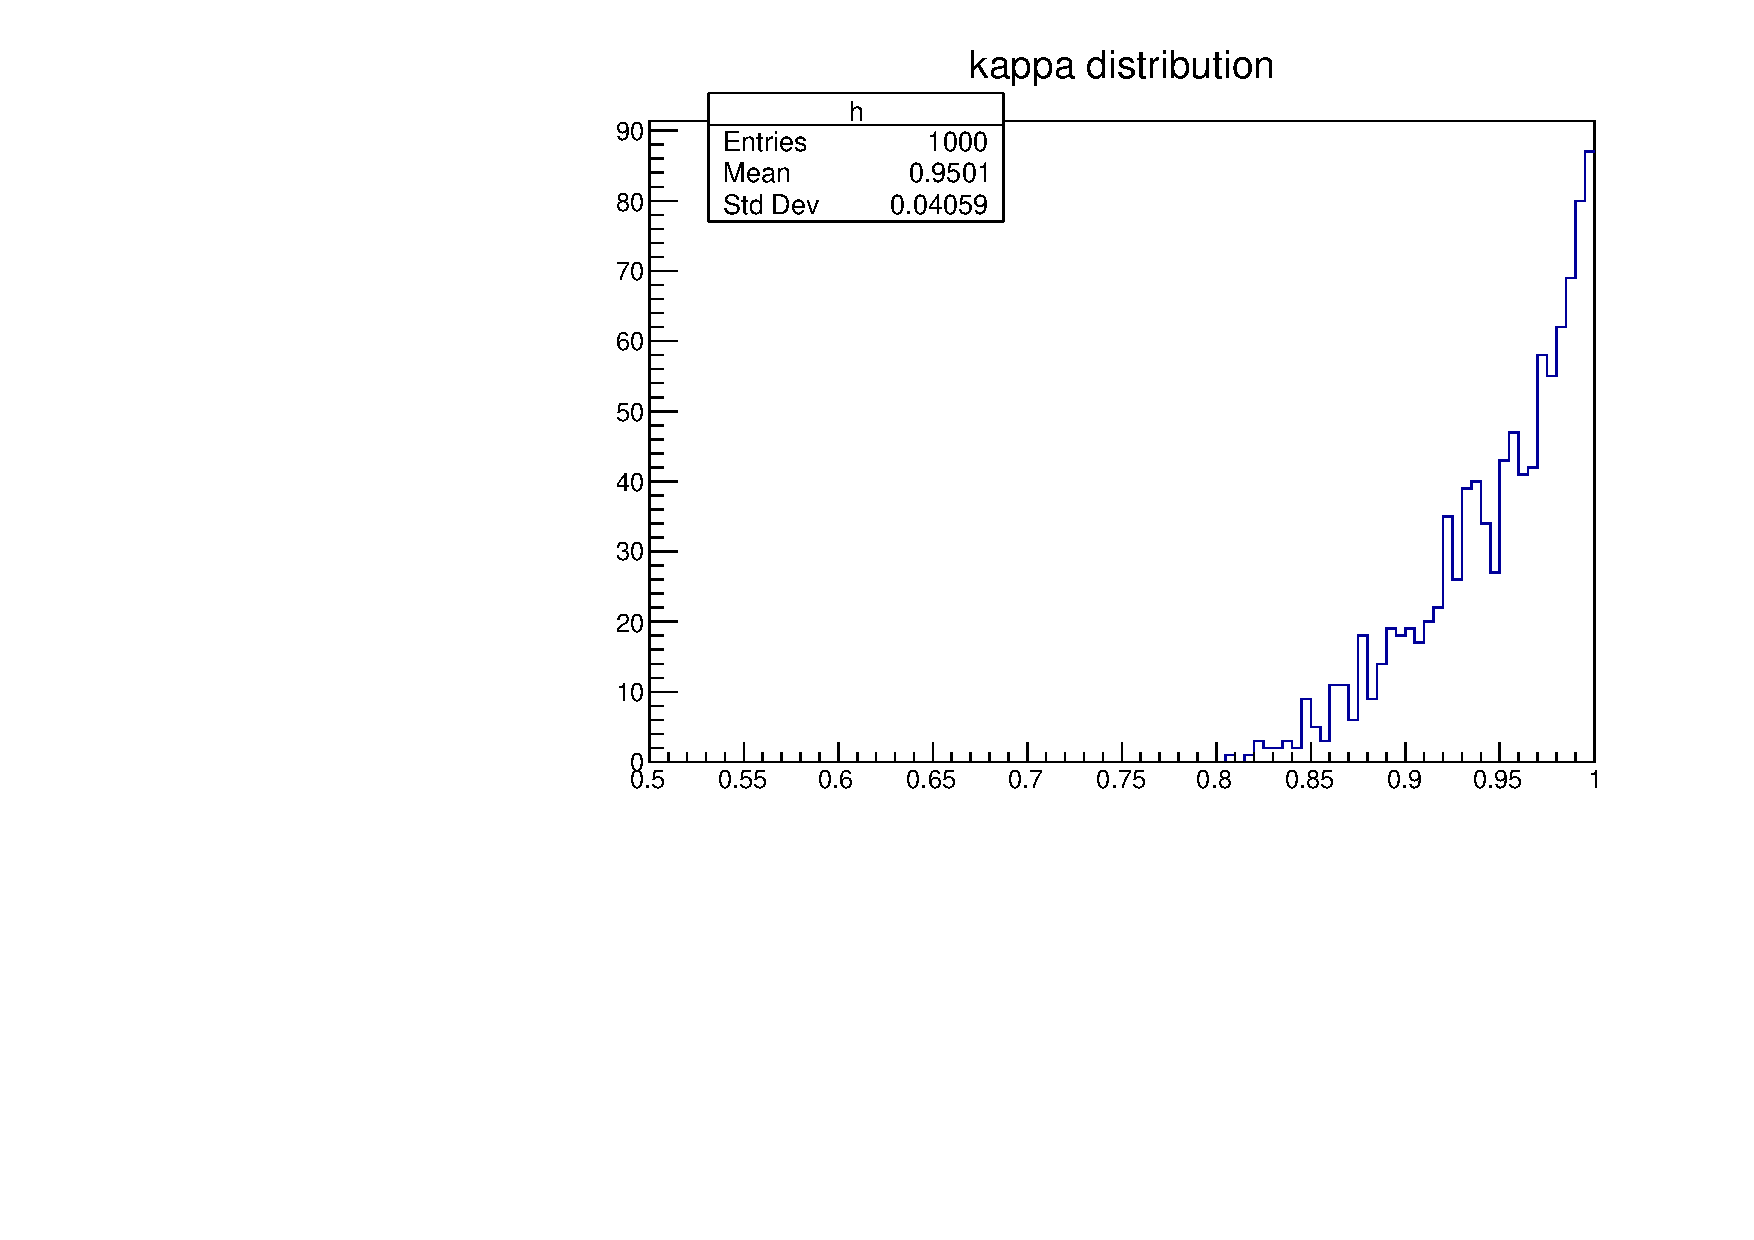
\includegraphics[width=0.5\linewidth]{figures/results/kappa.pdf}
\caption{Distribution of the measurements of $\kappa$ from 1000 toys}
\label{kappadistribution}
\end{figure}

\section{External inputs}
\label{sec:interpretation:inputs}

Several external inputs are required to interpret the results of the \CP observables from the \CP fit into information on $r_B$, $\delta_B$ and \Pgamma. The external parameters required are $r_D^{K\pi}$, $\delta_D^{K\pi}$, $r_D^{K3\pi}$, $\delta_D^{K3\pi}$, $\kappa_{4\pi}$ and $\kappa_{K3\pi}$. The parameters $\kappa_{4\pi}$ and $\kappa_{K3\pi}$ are to account for the fact that the four-body modes are not pure \CP or pure ADS modes. These parameters are measured in terms of the fractional \CP content of the decay \decay{\Dz}{\pip\pim\pip\pim}, $F_{CP}$, where $\kappa_{4\pi} = 2F_{CP} - 1$, and the coherence factor for the \decay{\Dz}{\Km\pip\pim\pip} decay, $R_{K3\pi} = \kappa_{K3\pi}$. These inputs $F_{CP}$ and $R_{K3\pi}$ are measurements taken from CLEO and LHCb measurements in Ref.~\cite{charmk3pi,LHCb-PAPER-2015-057,charm4pi}. The interpretation of \lhcb results depends on \lhcb acceptance across the four-body phase space. This effect is expected to be negligible.

Figures \ref{dalitzk3pi} and \ref{dalitz4pi} show plots of projections of the four-body phase space distributions for $K\pi\pi\pi$ and $\pi\pi\pi\pi$ respectively. These plots are comparisons of distributions for simulated generator level distributions without any acceptance effects and fully reconstrcuted selected MC events in my analysis. These distributions are shown to be very similar, which suggests that the use of the $K\pi\pi\pi$ coherence factor, $R_{K3\pi}$, and fractional \CP content, $F_{CP}$, from CLEO can be used directly in the interpretation of \lhcb results.  

\begin{figure}[h]
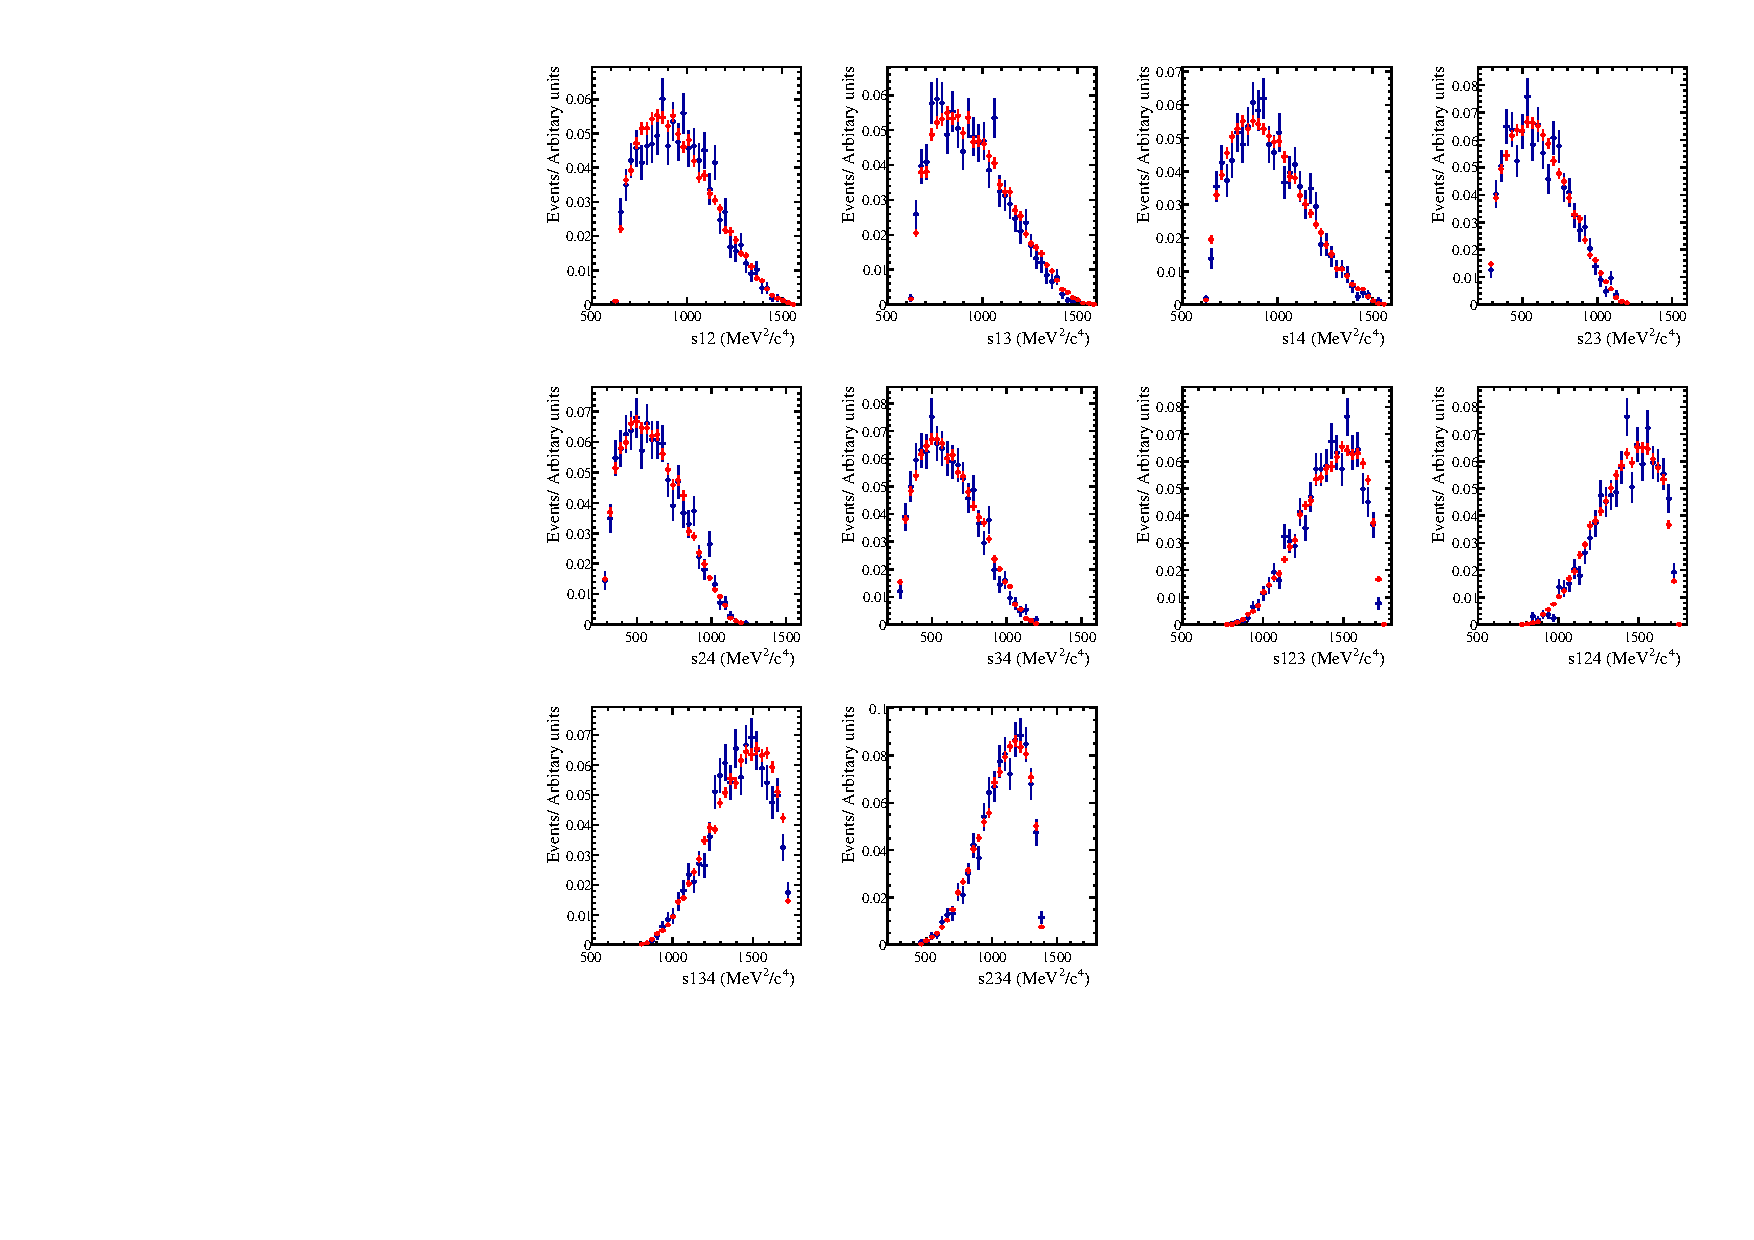
\includegraphics[width=\linewidth]{figures/results/dalitzDist_KPiPiPi.pdf}
\caption{Comparison of Dalitz variable distributions for simulation of generator level distributions (blue) and fully reconstructed selected events (red) in the $K\pi\pi\pi$ mode.}
\label{dalitzk3pi}
\end{figure}

\begin{figure}[h]
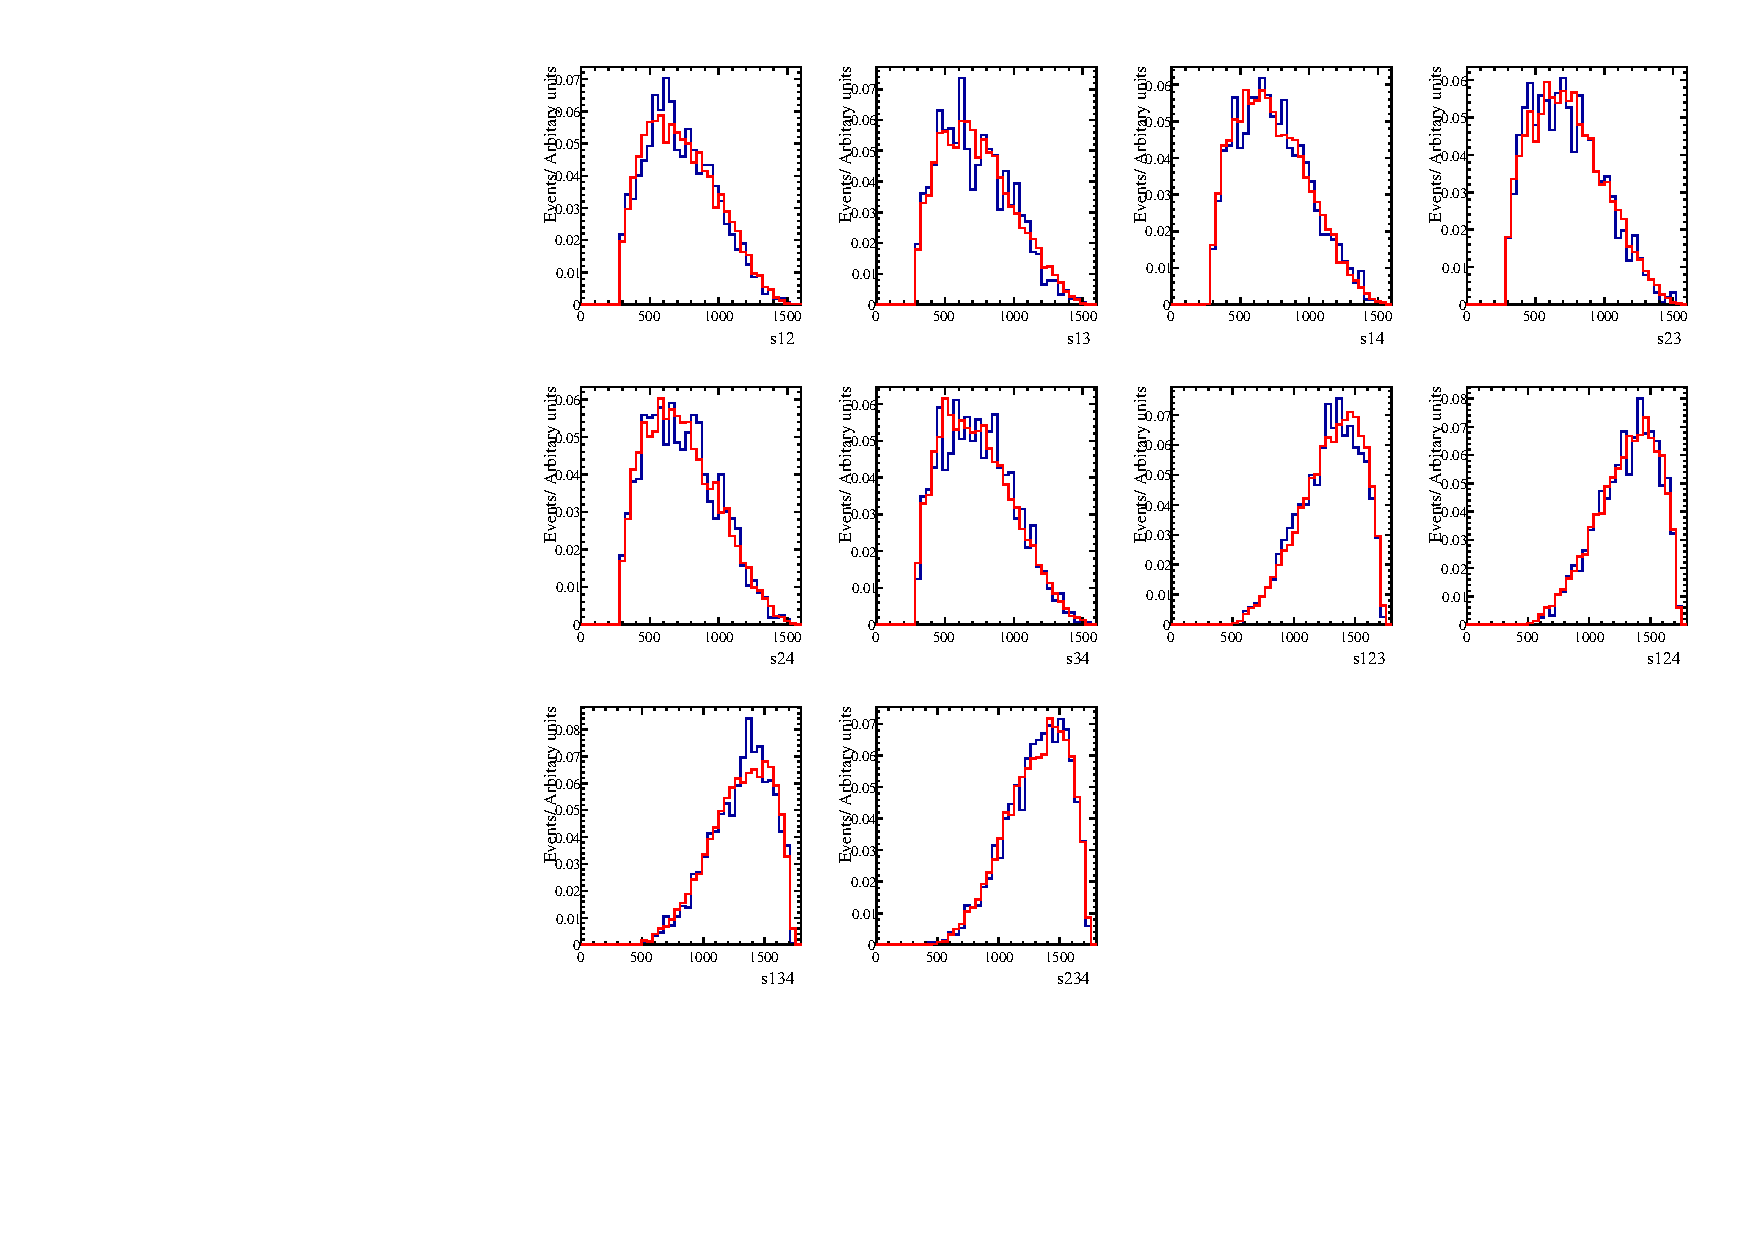
\includegraphics[width=\linewidth]{figures/results/dalitzDist_PiPiPiPi.pdf}
\caption{Comparison of Dalitz variable distributions for simulation of generator level distributions (blue) and fully reconstructed selected events (red) in the $\pi\pi\pi\pi$ mode.}
\label{dalitz4pi}
\end{figure}

The phase-space acceptance profile is primarily driven by the trigger, and then to some extent by the PID requirements. The effect of the BDT selection in relation to these is small. Hence it is expected that the phase-space acceptance profiles of the \decay{\D}{K\pi\pi\pi} and \decay{\D}{\pi\pi\pi\pi} decay modes in this analysis matches that of the \decay{\Bpm}{\D h^{\pm}} analysis. Hence it can be assumed that the same alterations to the interpretation are required as for the \decay{\Bpm}{\D h^{\pm}} analysis (no corrections for $R_{K3\pi}$ or $\delta_D^{K3\pi}$ and a small inflation of the uncertainty on $F_{CP}$). This assumption is verified in the studies detailed below.

\subsection{Effect of non-uniform acceptance on $R_{K3\pi}$ and $\delta_D^{K3\pi}$}

To assess the effects of small varaition in the four-body phase space for $K\pi\pi\pi$, the coherence factor and strong phase are calculated from the $K\pi\pi\pi$ amplitude models, as for the \decay{\Bpm}{\D h^{\pm}} analysis~\cite{B2DK_ADSGLW} using the AmpGen package, under the assumption of uniform acceptance and under the assumption of the total \lhcb acceptance. The differences give an estimate of the corrections that should be applied to the CLEO result before it is used in the \lhcb interpretation. The difference between the two was calculated to be 0.002 for the coherence factor and 0.7$^{\circ}$ for the strong phase difference, which are similar to the \decay{\Bpm}{\D h^{\pm}} analysis~\cite{B2DK_ADSGLW}. The values of the inputs taken from CLEO/LHCb are $R_{K3\pi} = 0.43^{+0.17}_{-0.13}$ and $\delta_D^{K3\pi} = \left(128^{+28}_{-17}\right)$~\cite{charmk3pi}. The size of the shifts due to the \lhcb phase space acceptance are negligible in comparison to the CLEO uncertainties and hence no further action is taken.

\subsection{Effect of non-uniform acceptance on $F_{CP}$}

When using an external value of $F_{CP}$ in this analysis~\cite{charm4pi} it is necessary to consider the potential distortion of the \lhcb acceptance. The acceptance will suppress certain regions of 4$\pi$ phase space, which may contain particular intermediate resonances, thus changing the overall CP content of the mode. Here we consider the approach taken in the \decay{\Bpm}{\D h^{\pm}} analysis, details of which can be found in LHCb-ANA-2014-071~\cite{B2DK_ADSGLW}, which involves determining the binned \lhcb acceptance and using it to reweight the CLEO-c data. The fit for $F_{CP}$ is then rerun on the weighted CLEO-c data and the difference in central values is used to get an idea of how the \lhcb acceptance might distort the true value of that parameter.

In this analysis we calculate the normalised binned \lhcb acceptance to compare with the results from the \decay{\Bpm}{\D h^{\pm}} analysis. In the \decay{\Bpm}{\D h^{\pm}} analysis the kinematic variables chosen to determine the \lhcb acceptance were the momentum and polar angle ($\theta$) of each pion in the \D rest frame. The acceptance is then measured in different bins of momentum and $\theta$ using simulated \decay{\Bpm}{\D(4\pi)\pipm} decays. The acceptance in each bin is defined to be ratio of the simulated \decay{\Bpm}{\D(4\pi)\pipm} sample with all selection applied to simulated generator level sample produced without any acceptance cuts. The acceptance is normalised because it is the bin-to-bin differences that are important. Exactly the same procedure is implemented in this analyis. The binning scheme used in both cases is (numbered 1-4 from low to high):

\begin{itemize}
\item Momentum: 0.0-0.3, 0.3-0.5, 0.5-0.7, 0.7-1.0 \gevcc
\item $\theta$: 0.30-1.00, 1.00-1.50, 1.50-2.00, 2.00-2.70 radians
\end{itemize}

The reconstruction and generator level distributions are shown in Figure \ref{acceptance} and the normalised acceptance in each bin is given in Table \ref{normalisedacceptance}.

\begin{figure}[h]
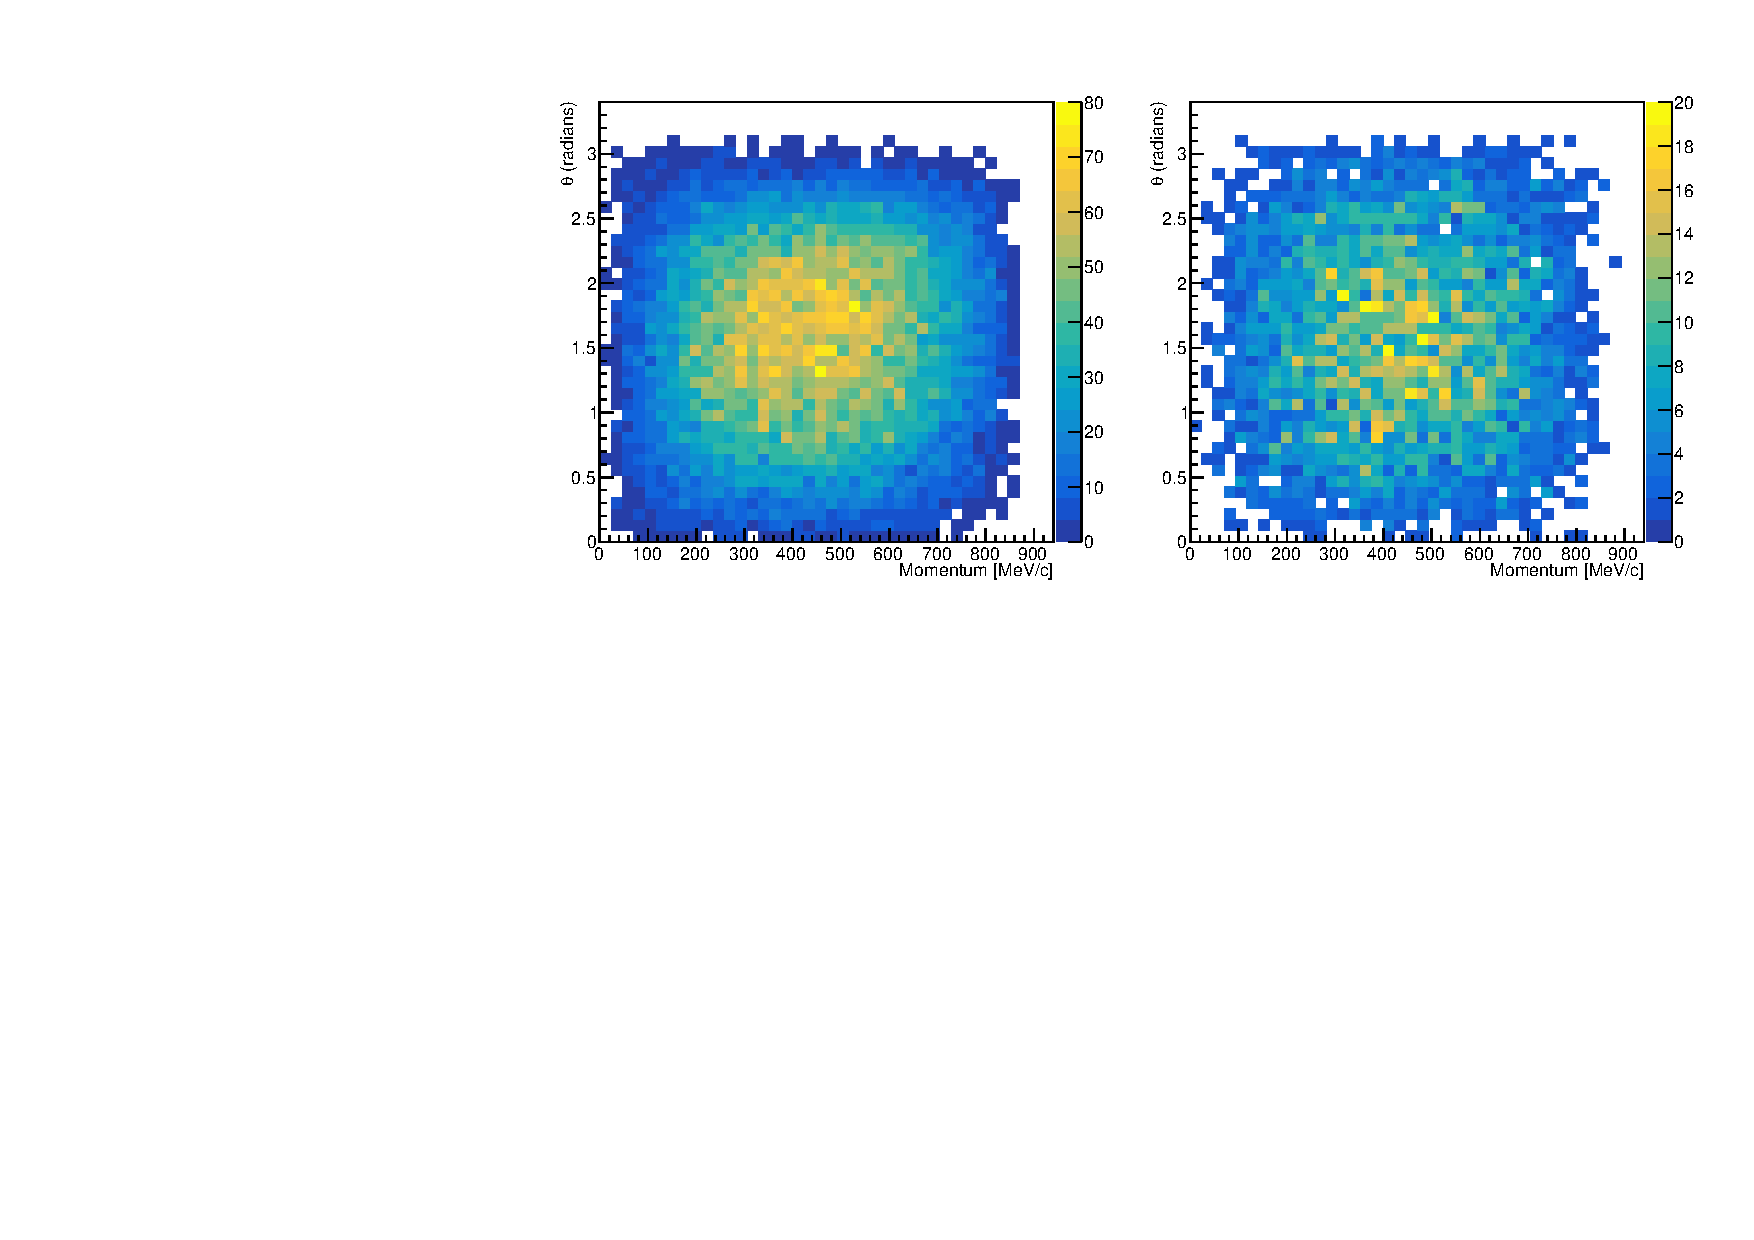
\includegraphics[width=\linewidth]{figures/results/acceptance4pi.pdf}
\caption{Reconstruction (left) and generator level (right) distributions of \lhcb sample of simulated \decay{\Bpm}{\D(4\pi)\Kstarpm} decays.}
\label{acceptance}
\end{figure}

\begin{table}
\centering
\begin{tabular}{c|cccc}
& \multicolumn{4}{c}{Momentum bin} \\
\hline
$\theta$ bin & 1 & 2 & 3 & 4 \\ 
\hline
4 & $0.76 \pm 0.30$ & $0.92 \pm 0.26$ & $0.90 \pm 0.24$ & $1.0 \pm 0.3$ \\ 
3 & $1.1 \pm 0.4$ & $0.88 \pm 0.24$ & $0.90 \pm 0.23$ & $1.0 \pm 0.3$ \\ 
2 & $1.4 \pm 0.5$ & $1.0 \pm 0.3$ & $1.0 \pm 0.3$ & $1.1 \pm 0.3$ \\ 
1 & $1.1 \pm 0.4$ & $1.2 \pm 0.3$ & $0.94 \pm 0.24$ & $0.88 \pm 0.25$ \\
\end{tabular}
\caption{Normalised acceptance for the \lhcb sample of simulated \decay{\Bpm}{\D(4\pi)\Kstarpm} decays. The bins are presented in the orientation shown in Figure \ref{acceptance}.}
\label{normalisedacceptance}
\end{table}

The results in Table \ref{normalisedacceptance} are consistent with the \decay{\Bpm}{\D(4\pi)\pipm} results~\cite{B2DK_ADSGLW}, therefore it is considered sufficient to apply the result of the \decay{\Bpm}{\D(4\pi)\pipm} procedure to this analysis. In the \decay{\Bpm}{\D h^{\pm}} analysis, it is concluded that increasing the total uncertainty of $F_{CP}$ from 0.028 to 0.034 accounts for any uncertainty due to non-uniform \lhcb acceptance. Therefore, the value of $F_{CP}$ used as an input when determining $r_B$, $\delta_B$ and \Pgamma is $0.734 \pm 0.034$.

\section{Results in terms of $r_B$, $\delta_B$ and \Pgamma}
\label{sec:interpretation:gammadini}

The physics observables can be used to get a handle on the physics parameters of interest: $r_B$, $\delta_B$ and \Pgamma. 
The results of the physics observables in the \CP fit, given in Table \ref{cpfitresultsphysics}, can be related to the physics parameters via Equations ~\ref{exp_Acp} - ~\ref{exp_Rpm4body}. The coherence factor is used as determined in the previous section. Further external parameters are required are $r_D^{K\pi}$, $\delta_D^{K\pi}$, $r_D^{K3\pi}$, $\delta_D^{K3\pi}$, $\kappa_{4\pi}$ and $\kappa_{K3\pi}$. The parameters $\kappa_{4\pi}$ and $\kappa_{K3\pi}$ are to account for the fact that the four-body modes are not pure \CP or pure ADS modes. These parameters are measured in terms of the fractional \CP content of the decay \decay{\Dz}{\pip\pim\pip\pim}, $F_{CP}$, where $\kappa_{4\pi} = 2F_{CP} - 1$, and the coherence factor for the \decay{\Dz}{\Km\pip\pim\pip} decay, $R_{K3\pi} = \kappa_{K3\pi}$. For all these HFAG provides the latest values, uncertainties and correlations.
The physics observables and other parameters are combined using the gammadini package. This framework performs a minimisation. The physics parameters involved are $r_B, \delta_B, \gamma, \kappa, r_D^{K\pi}, \delta_D^{K\pi}, r_D^{K3\pi}, \delta_D^{K3\pi}, \kappa_{4\pi}, \kappa_{K3\pi}$ where $\kappa, r_D^{K\pi}, \delta_D^{K\pi}, r_D^{K3\pi}, \delta_D^{K3\pi}, \kappa_{4\pi}, \kappa_{K3\pi}$ are constrained to their determined/measured values. 
A global $\chi^2$ minimisation is performed where
\begin{equation}
\chi^2 = \sum_i \chi^2_i = (x(\theta) - x_0)^TV_0^{-1}(x(\theta)-x_0)
\end{equation}
In this expression, $x(\theta)$ is the set of observables caluculated from the fundamental set of paraemters $\theta$ and $x_0$ are the measured values. $V_0$ is the covariance matrix.
The sensitivity of a given parameter is determined by calculating the $\chi^2$ at fixed points in parameter space. The difference between this $\chi^2$ value and that of the global minimum, quantifies the confidence in the global minimum. 

The results of the fit parameters is shown in Table \ref{gammadinifit}. Figures \ref{gammadiniplots2body} and \ref{gammadiniplotsallmodes} give the results as 2D contour plots of $r_B$ versus \Pgamma and $\delta_B$ versus \Pgamma. Figure \ref{gammadiniplots2body} shows the contour plots using the two-body modes only and Figure \ref{gammadiniplotsallmodes} show the contour plots using the observables from both the two- and four-body decays. The addition of the four-body modes slight improves the constraints on the physics parameters, but in particular it provides additional distinction between the two minima. The nominal expected value of $\gamma \sim 70^\circ$ is consistent with the data at less than $2\sigma$. As expected by assuming $\gamma=70^\circ$ there is a solution of $\delta_B$ that is consistent with being small and in the first quadrant. The preferred value of $r_B$ is also quite consistent with expectation of being similar to that of $B \to DK \sim 0.1$.

Calculating the values of $r_B$, $\delta_B$ and \Pgamma from running 100 pseudoexperiments gives values of:
\begin{align*}
r_B &= 0.116^{+0.015}_{-0.019} \\
\delta_B &= \left(40.4^{+17.0}_{-17.0}\right)^{\circ} \\
\Pgamma &= \left(39.8^{+19.0}_{-16.0}\right)^{\circ} 
\end{align*}

These confidence level distributions for $r_B$, $\delta_B$ and \Pgamma are not Gaussian beyond 1$\sigma$ and $\delta_B$ and \Pgamma contain another minimum, as can be seen from Figure \ref{gammadiniplotsallmodes}, therefore the results quoted cannot be extrapolated to consider 2$\sigma$ or 3$\sigma$ values. 

\begin{figure}[h]
\centering
\subfloat[$r_B$ versus \Pgamma]{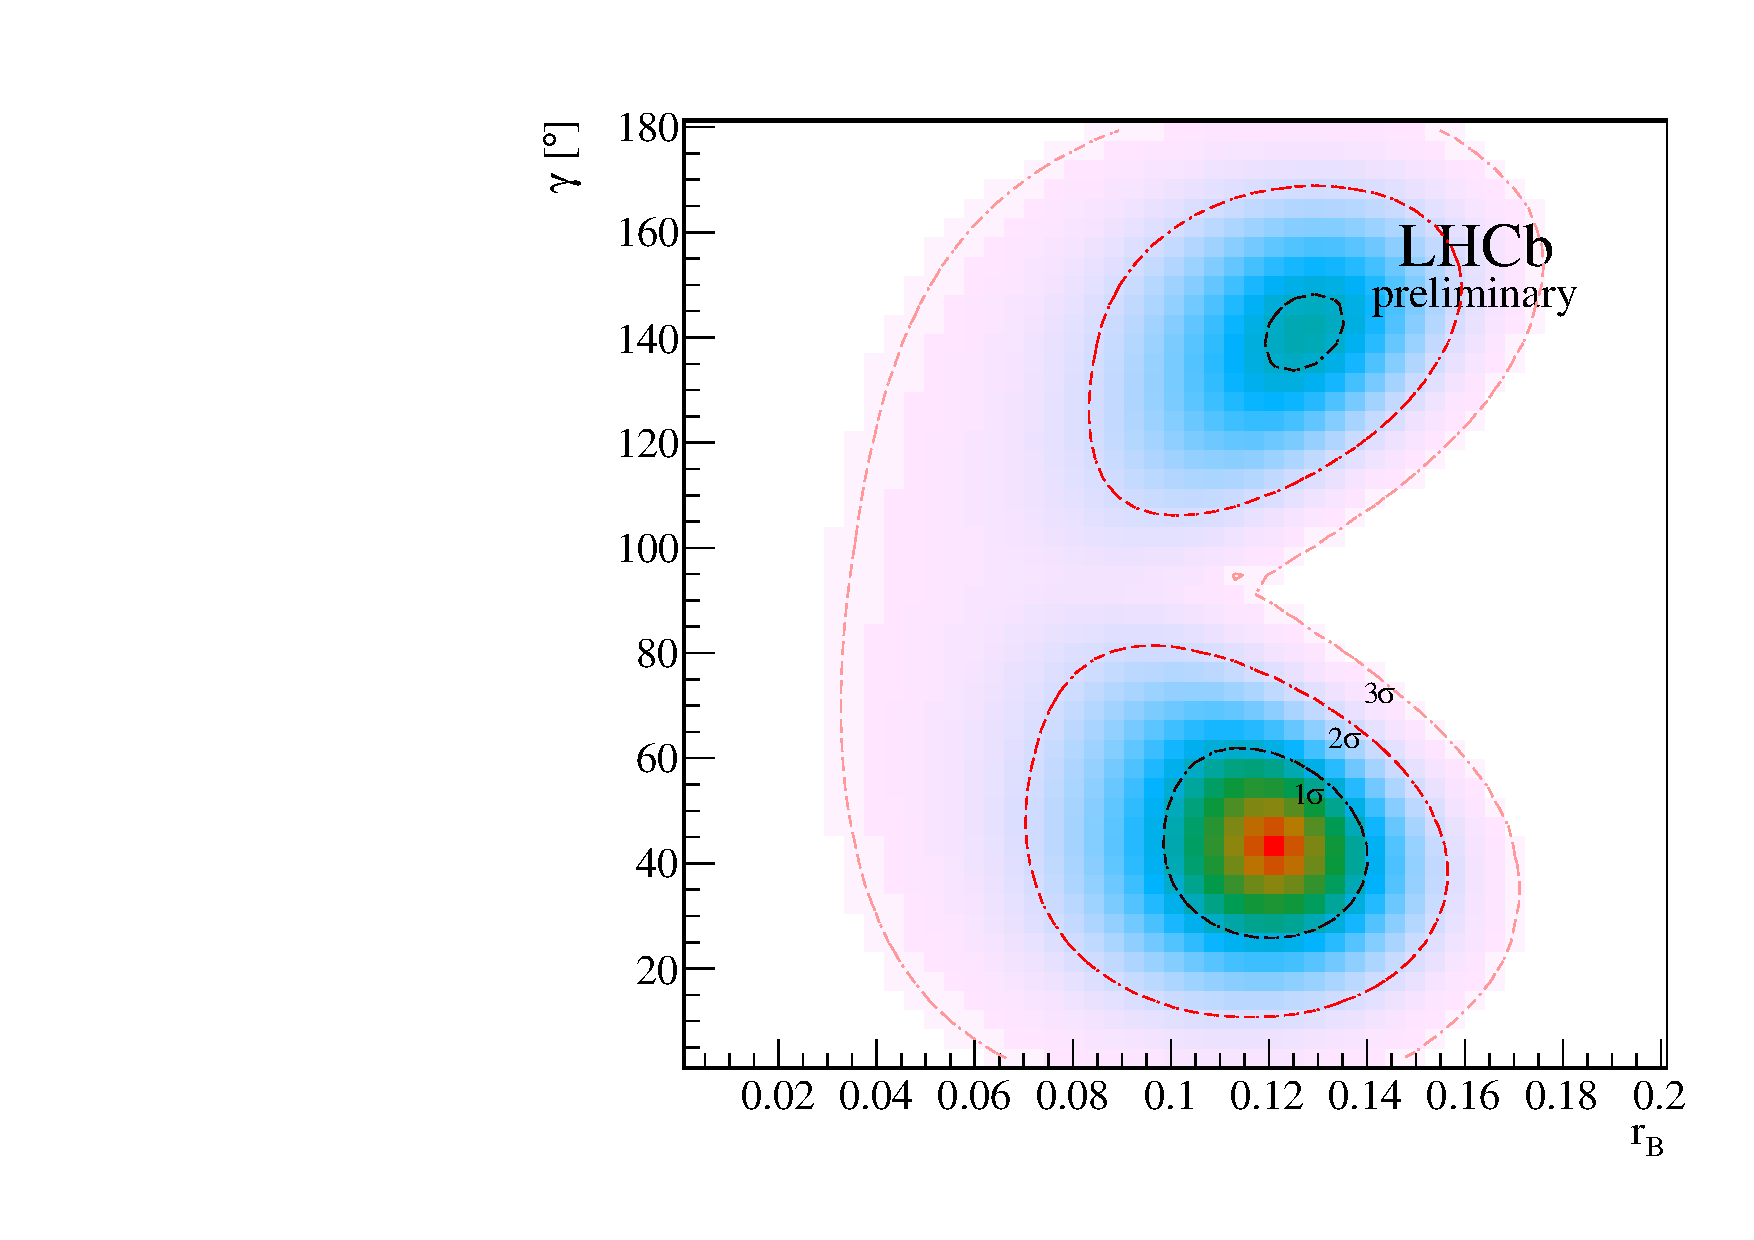
\includegraphics[width=0.5\linewidth]{figures/results/rBu_dkstar_gamma_2Dscan_nomixing_2body.pdf}}
\subfloat[$\delta_B$ versus \Pgamma]{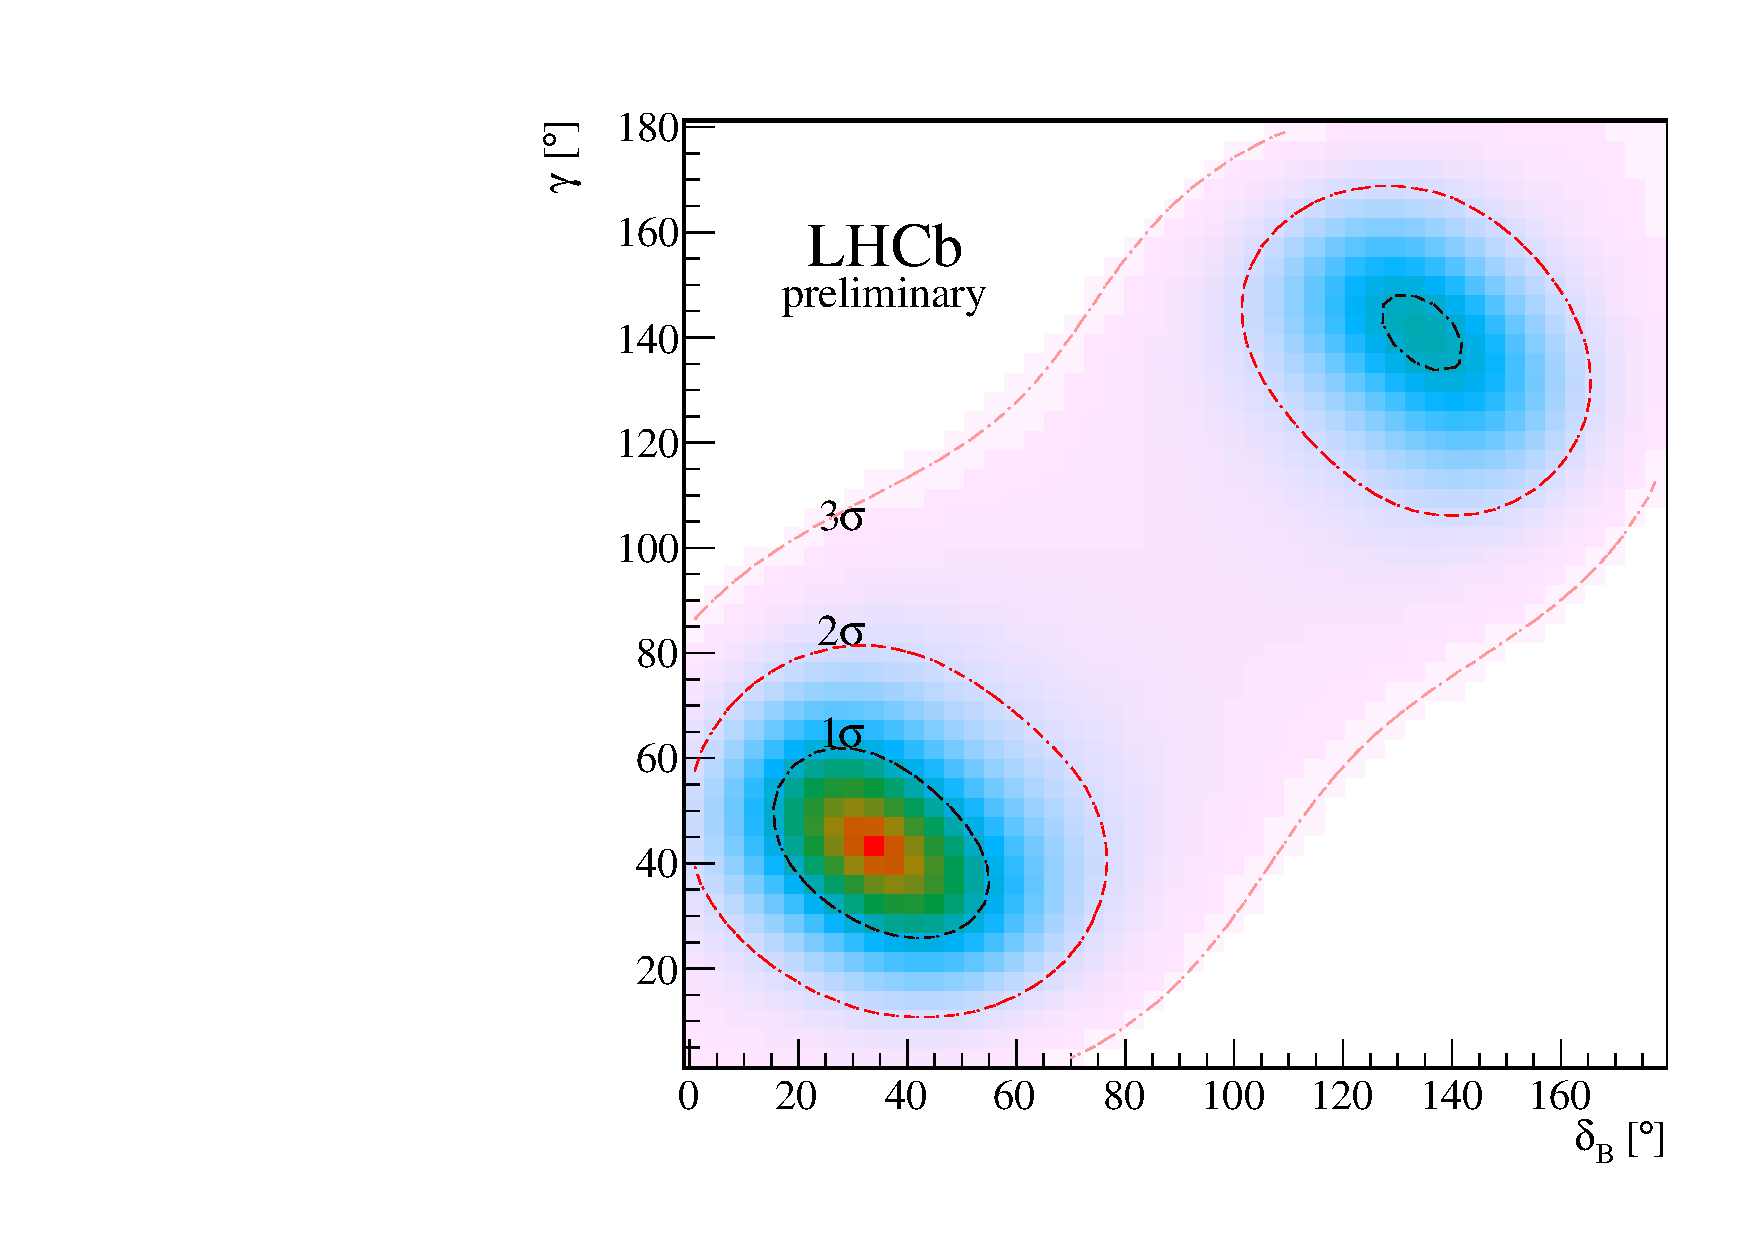
\includegraphics[width=0.5\linewidth]{figures/results/deltaBu_dkstar_gamma_2Dscan_nomixing_2body.pdf}}
\caption{2D contour plots using the two-body modes only}
\label{gammadiniplots2body}
\end{figure}

\begin{figure}[h]
\centering
\subfloat[$r_B$ versus \Pgamma]{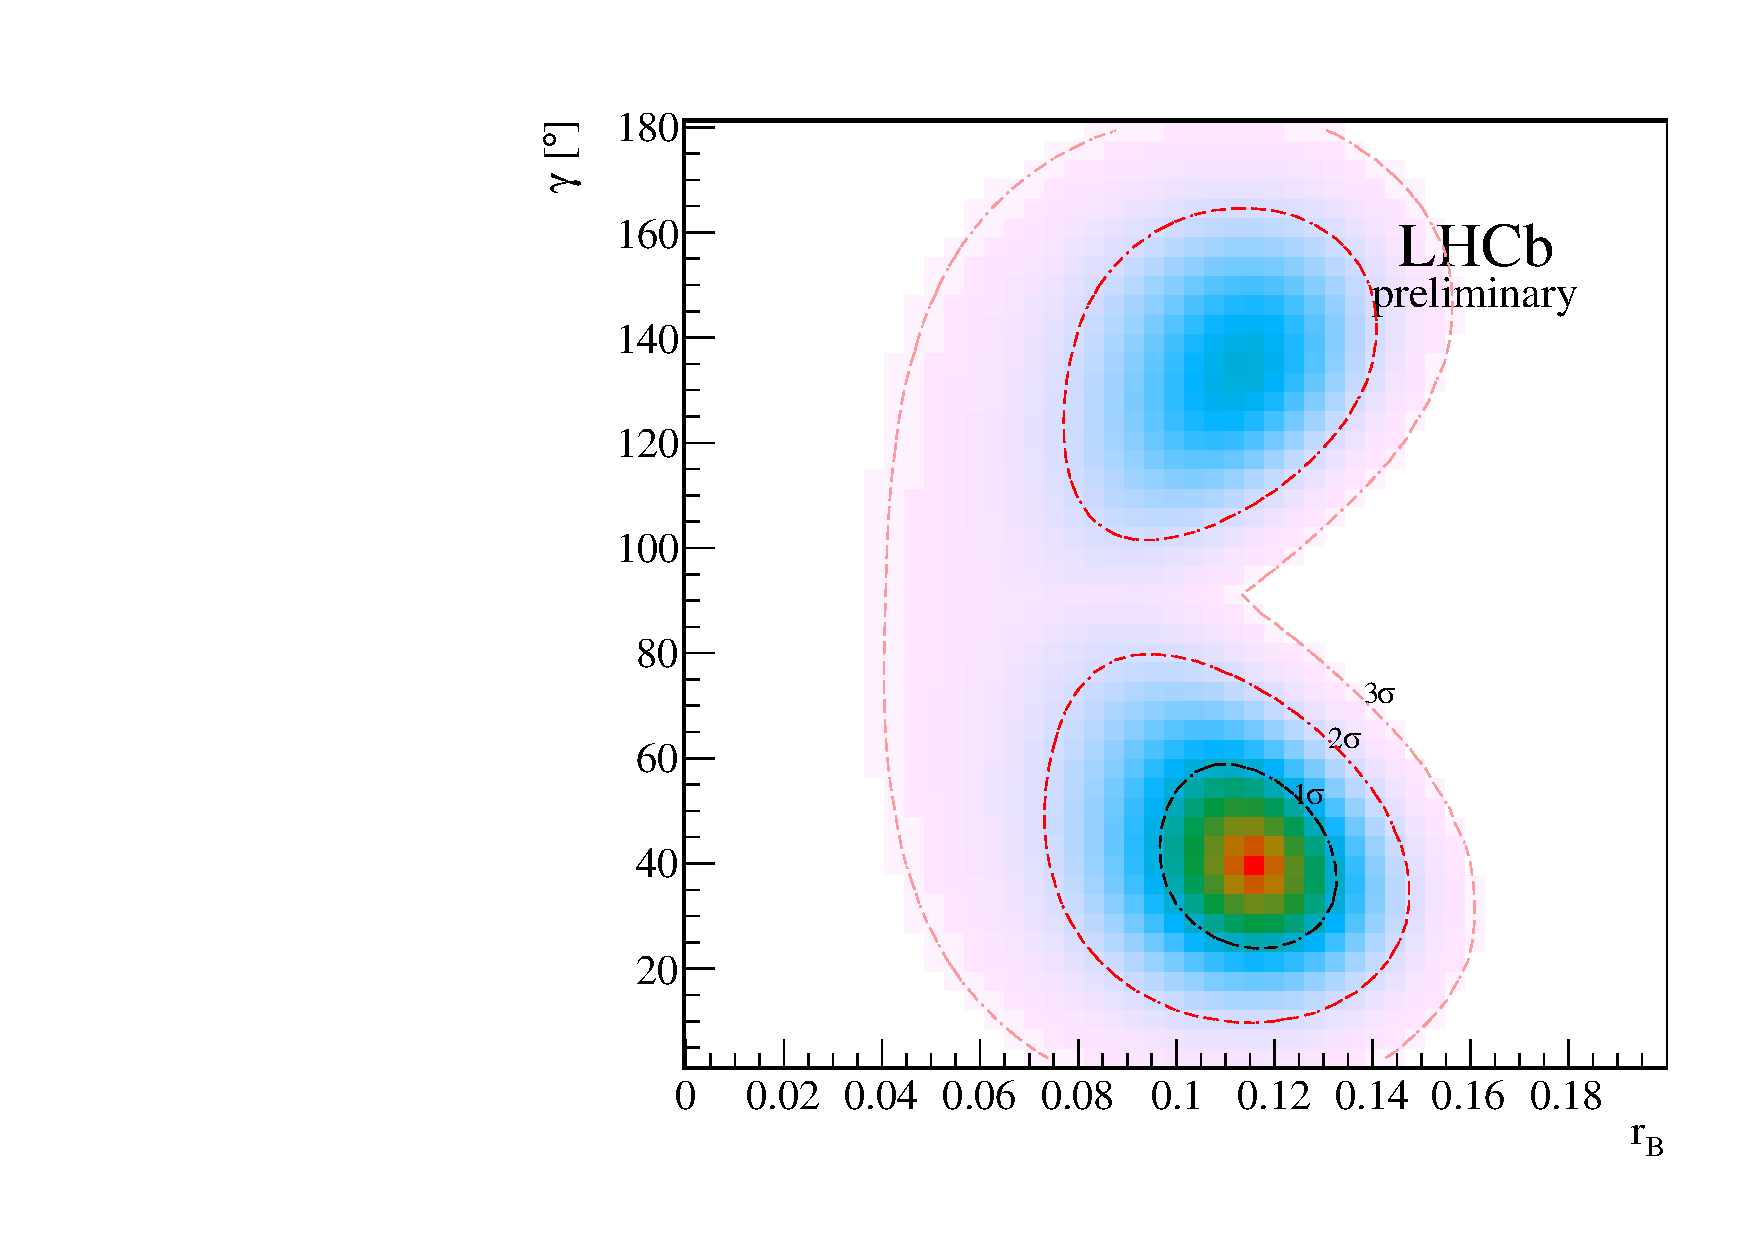
\includegraphics[width=0.5\linewidth]{figures/results/rBu_dkstar_gamma_2Dscan_nomixing.pdf}}
\subfloat[$\delta_B$ versus \Pgamma]{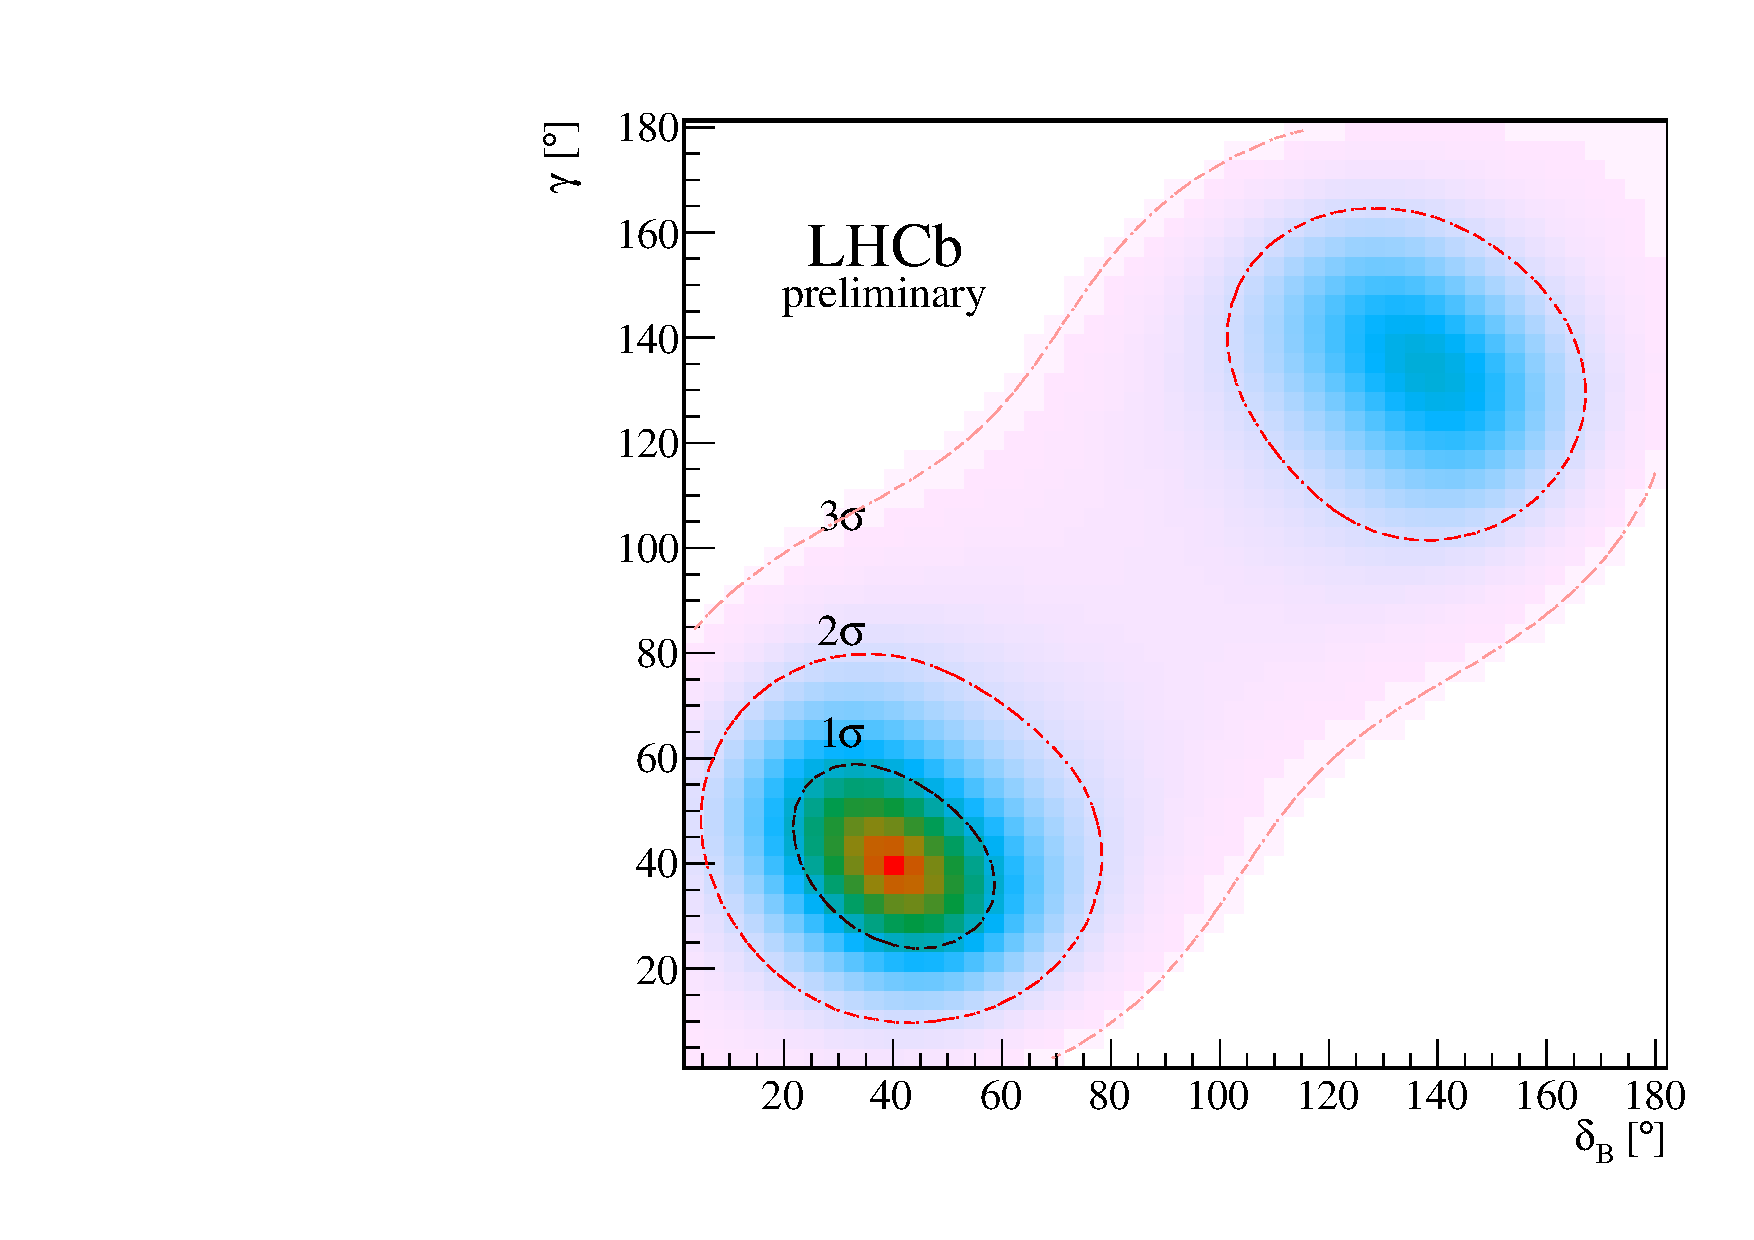
\includegraphics[width=0.5\linewidth]{figures/results/deltaBu_dkstar_gamma_2Dscan_nomixing.pdf}}
\caption{2D contour plots using both the two- and four-body modes}
\label{gammadiniplotsallmodes}
\end{figure}

\begin{table}
\centering
\begin{tabular}{cccc}
Fit parameter & Value & Negative error & Positive error \\
\hline
\Pgamma & 40 & -16 & 19 \\
$r_B$ & 0.116 & -0.019 & 0.017 \\
$\delta_B$ & 40 & -19 & 18 \\
$\kappa$ & 0.96 & -0.06 & 0.06 \\
$r_D^{K\pi}$ & 0.0591 & -0.0003 & 0.0003 \\
$\delta_D^{K\pi}$ & 193 & -11 & 11 \\
$r_D^{K3\pi}$ & 0.0549 & -0.0006 & 0.0006 \\
$\delta_D^{K3\pi}$ & 133 & -22 & 22 \\
$R_{K3\pi}$ & 0.44 & -0.15 & 0.15 \\
$F_{CP}$ & 0.74 & -0.03 & 0.03
\end{tabular}
\caption{Results of fit parameters}
\label{gammadinifit}
\end{table}


\clearpage
